\subsection{The Optimization Problem}
The basic scheme for the optimization problem is given in \figref{SensToolSchema}.
%
\begin{figure}[H]
	\centering
	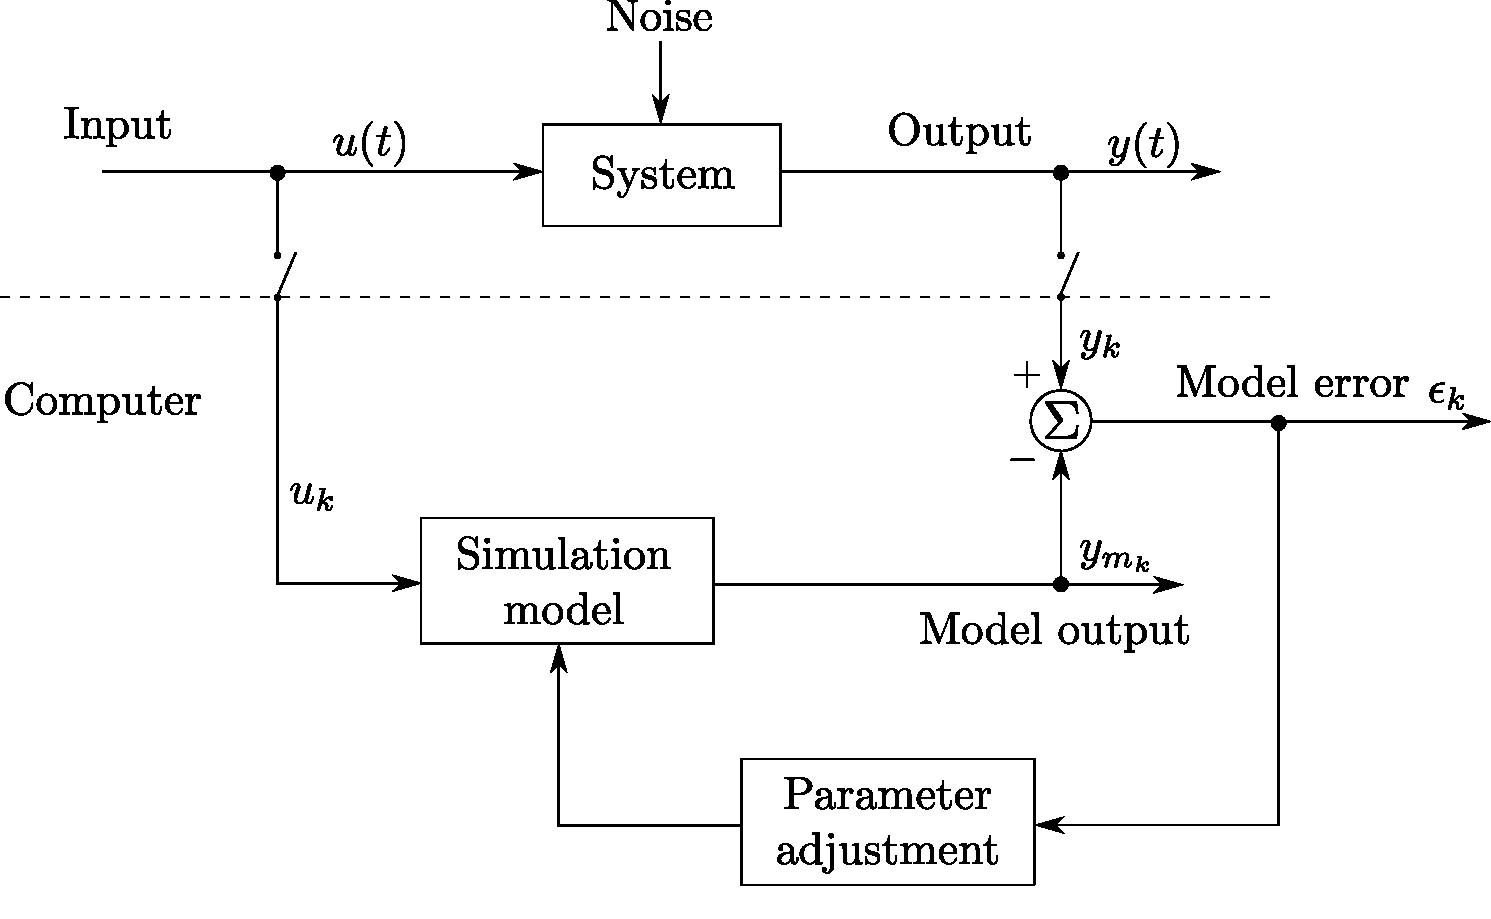
\includegraphics[scale=0.4]{figures/senstoolsModelOptimizationHM}
%	\input{figures/schematicSensTool.tikz}
%	\centering
	\caption{Schematic of the optimization problem, where input (u(t)) and output(y(t)) data is logged. The input data is used with the simulation to generate the simulation output (\si{y_{m}(t)}). The real output and the simulated output are then compared and an adjustment is made to the parameters of the simulation. Then a new \si{y_{m}(t)} is generated with the u(t) and compared to the y(t). This process is iterated until a satisfactory match between y(t) and \si{y_{m}(t)} is achieved. Inspired from Senstools documentation.\cite{Senstools}.}
	\label{SensToolSchema}
\end{figure}
%
The provided data is taken from an initial value test of the Cubli hanging down like a pendulum, see \appref{app:impulseResponseAppendix}.
If the fit is done in the operating region from \si{-0,15\ to\ 0,15\ rad}, the simulated behavior in this range will be closer to reality.

Furthermore, the nonlinear model is used to accurately describe the oscillatory behavior of the pendulum. The model is modified such that it describes the system as a regular pendulum without the dynamics of the reaction wheel, in order to match the test conditions under which the data was extracted, as seen in \figref{blockDiagramSenseTool}.
%
\begin{figure}[H]
	  \begin{tikzpicture}[ auto,
                       thick,                         %<--setting line style
                       node distance=1.5cm,             %<--setting default node distance
                       scale=0.75,                     %<--|these two scale the whole thing
                       every node/.style={scale=0.62}, %<  |(always change both)
                       >/.tip={Triangle[angle=40:5pt]}
                       ]

    %-- Blocks creation --%
    \draw
      % DIRECT TERM %
      node[shape=coordinate][](input1) at (0,0){}
      node[shape=coordinate][](feedForward) at (0.5,0){}
      node(sum1) at (2.25,0) [sum]{\si{\sum}}
      node(sum2) at (3.75,0) [sum]{\si{\sum}}

      node(torque2rotacc1) at (6.85,0) [block]{\large \si{\frac{1}{J_F + J_w + m_w \cdot {l_w}^{2}}}}

      node(integration1) at (10.75,0) [block] {\large \si{\frac{1}{s}}}
      node(integration2) at (14.2,0) [block] {\large \si{\frac{1}{s}}}

      node[shape=coordinate][](output) at (15.3,0){}
      node[shape=coordinate][](veloFeedbackNode) at (11.8,0){}
      
    ;
    \draw
      % FEEDBACKS %
      node(veloFeedback) at (7,-2) [block] {\large \si{B_F}}
      node(angleFeedback) at (8,-4) [block] {\large \si{(m_F \cdot l_F + m_w \cdot l_w)g}}
    ;
    %-- Block linking --%
    % INPUT %
    \draw[-](input1)        -- node{\large \si{\tau_m(s)}}(feedForward);
    \draw[->](feedForward)  -- (sum1);

    % OUTPUT %
    \draw[-](integration2)  -- (output);
    \draw[->](output)       -- node {\large \si{\theta_{F}(s)}} (17,0);

    % DIRECT TERM %
    \draw[->] (sum1)            -- (sum2);
    \draw[->] (sum2)            -- (torque2rotacc1);
    \draw[->] (torque2rotacc1)  -- node{\large \si{\alpha_F(s)}}(integration1);
    \draw[->] (integration1)    -- node{\large \si{\omega_F(s)}}(integration2);

    % FEEDBACKS

    \draw[->] (output)           |- (angleFeedback);
    \draw[->] (angleFeedback)    -| (sum1);

    \draw[->] (veloFeedbackNode) |- (veloFeedback);
    \draw[->] (veloFeedback)     -| (sum2);

    %-- Nodes --%
    \draw%--------------------------------------------------------------
      node at (input1)            [shift={(-0.04, -0.05 )}] {\Large \textopenbullet}
      node at (output)            [shift={( 0.007, -0.05 )}] {\Large \textbullet}
      node at (veloFeedbackNode)  [shift={( 0.007, -0.05 )}] {\Large \textbullet}
    ;

    %-- Summation signs --%
      \draw%--------------------------------------------------------------

      node at (sum1) [right = -6.6mm, below = .6mm] {$-$}
      node at (sum1) [right = -3mm, below = 3.9mm]  {$+$}
      node at (sum2) [right = -6.6mm, below = .6mm] {$+$}
      node at (sum2) [right = -3mm, below = 3.9mm]  {$-$}

    ;

  \end{tikzpicture}
	\centering
	\caption{Block diagram of the system as a regular pendulum with the wheel fixed to the frame.}
	\label{blockDiagramSenseTool}
\end{figure}
%
In order to minimize the difference between the data points measured in test and the output of the model, a function to describe such a relationship is needed. The cost function used to describe goodness of the fit, is a mean square error function.
%
\begin{flalign}
	\eq{P(\vec{\theta})} {\frac{1}{2N}\sum_{k = 1}^{N} \left(y_{k} - y_{m_k}(\vec{\theta})\right)^2 } &
\label{costFunctionEquation}
\end{flalign}
%
\hspace{6mm} Where:\\
\begin{tabular}{ p{1cm} l p{10cm} l}
& \si{\vec{\theta}}   & is the parameter(s) to be adjusted                                                                      & \\
& \si{N}              & is the degrees of freedom for each parameter                                                            & \\
& \si{k}              & is each sample in time, \si{t=1T,\ 2T,\ } ...\si{,\ kT, } ...\si{,\ NT}\newline
                        where \si{T} is sampling time                                                                           & \\
& \si{{y}_{k}}        & is the \si{k^{th}} sample of the test measurement output vector                                         & \\
& \si{{y_{m_k}}}      & is the \si{k^{th}} sample of the model output vector                                                    & \\
\end{tabular}

A normal mean square error function is only divided by the degrees of freedom, \si{N}, but in this case it is divided by \si{2N} to cancel out the factor two which arises when computing its gradient. This does not have any impact on the solution since the minimum maintains its original position.